


\tikzset{every picture/.style={line width=0.75pt}} %set default line width to 0.75pt        

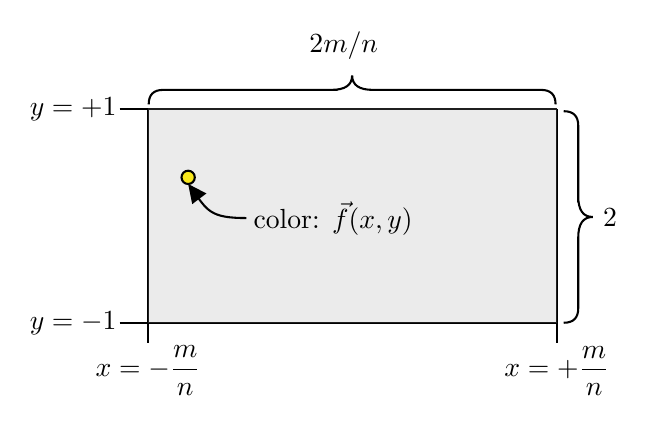
\begin{tikzpicture}[x=0.75pt,y=0.75pt,yscale=-1,xscale=1]
%uncomment if require: \path (0,207); %set diagram left start at 0, and has height of 207

%Shape: Brace [id:dp3485420546358562] 
\draw   (277.34,148.05) .. controls (282.01,148.05) and (284.34,145.72) .. (284.34,141.05) -- (284.34,107.08) .. controls (284.34,100.41) and (286.67,97.08) .. (291.34,97.08) .. controls (286.67,97.08) and (284.34,93.75) .. (284.34,87.08)(284.34,90.08) -- (284.34,53.12) .. controls (284.34,48.45) and (282.01,46.12) .. (277.34,46.12) ;
%Shape: Brace [id:dp32619366128453287] 
\draw   (273.42,42.85) .. controls (273.42,38.18) and (271.09,35.85) .. (266.42,35.85) -- (185.41,35.85) .. controls (178.74,35.85) and (175.41,33.52) .. (175.41,28.85) .. controls (175.41,33.52) and (172.08,35.85) .. (165.41,35.85)(168.41,35.85) -- (84.39,35.85) .. controls (79.72,35.85) and (77.39,38.18) .. (77.39,42.85) ;
%Straight Lines [id:da3020649451106543] 
\draw    (63.41,45.07) -- (274.08,45.07) ;
%Straight Lines [id:da561961885237614] 
\draw    (274.08,45.05) -- (274.08,157.85) ;
%Straight Lines [id:da7796723527373772] 
\draw    (77.13,44.81) -- (77.13,157.62) ;
%Straight Lines [id:da788223597357713] 
\draw    (63.41,148.31) -- (274.08,148.31) ;
%Shape: Rectangle [id:dp23965900795077655] 
\draw  [draw opacity=0][fill={rgb, 255:red, 155; green, 155; blue, 155 }  ,fill opacity=0.2 ] (77.13,44.81) -- (274.08,44.81) -- (274.08,148.31) -- (77.13,148.31) -- cycle ;
%Shape: Circle [id:dp5520249729432991] 
\draw  [fill={rgb, 255:red, 248; green, 231; blue, 28 }  ,fill opacity=1 ] (93.2,78) .. controls (93.2,76.23) and (94.63,74.8) .. (96.4,74.8) .. controls (98.17,74.8) and (99.6,76.23) .. (99.6,78) .. controls (99.6,79.77) and (98.17,81.2) .. (96.4,81.2) .. controls (94.63,81.2) and (93.2,79.77) .. (93.2,78) -- cycle ;
%Curve Lines [id:da6341583887995654] 
\draw    (98.2,83.65) .. controls (105.67,93.97) and (106.73,97.6) .. (124.4,97.6) ;
\draw [shift={(96.4,81.2)}, rotate = 52.98] [fill={rgb, 255:red, 0; green, 0; blue, 0 }  ][line width=0.08]  [draw opacity=0] (8.93,-4.29) -- (0,0) -- (8.93,4.29) -- cycle    ;

% Text Node
\draw (77.13,157.62) node [anchor=north] [inner sep=0.75pt]   [align=left] {$\displaystyle x=-\frac{m}{n}$};
% Text Node
\draw (274.08,157.85) node [anchor=north] [inner sep=0.75pt]   [align=left] {$\displaystyle x=+\frac{m}{n}$};
% Text Node
\draw (63.41,148.31) node [anchor=east] [inner sep=0.75pt]   [align=left] {$\displaystyle y=-1$};
% Text Node
\draw (63.41,45.07) node [anchor=east] [inner sep=0.75pt]   [align=left] {$\displaystyle y=+1$};
% Text Node
\draw (153.34,6.38) node [anchor=north west][inner sep=0.75pt]   [align=left] {$\displaystyle 2m/n$};
% Text Node
\draw (299.67,97.25) node   [align=left] {$\displaystyle 2$};
% Text Node
\draw (126.4,107.7) node [anchor=south west] [inner sep=0.75pt]   [align=left] {color: $\displaystyle \vec{f}( x,y)$};


\end{tikzpicture}